%%%%%%%%%%%%%%%%%%%%%%%%%%%%%%%%%%%%%%%%%%%%%%%%%%%%%%%%%%%%%%%%%%%%%%%%%%%%%%%
% Chapter 'Refrigerants - Nitrogen'
%%%%%%%%%%%%%%%%%%%%%%%%%%%%%%%%%%%%%%%%%%%%%%%%%%%%%%%%%%%%%%%%%%%%%%%%%%%%%%%
\section{Nitrogen}
%
%%%%%%%%%%%%%%%%%%%%%%%%%%%%%%%%%%%%%%%%%%%%%%%%%%%%%%%%%%%%%%%%%%%%%%%%%%%%%%%
%%%%%%%%%%%%%%%%%%%%%%%%%%%%%%%%%%%%%%%%%%%%%%%%%%%%%%%%%%%%%%%%%%%%%%%%%%%%%%%
\subsection{Saturated Liquid Density - EoS1 - ID 1}
%
\begin{tabular}[l]{|lp{11.5cm}|}
\hline
\addlinespace

\textbf{Name:} & Nitrogen \\
\textbf{Equation:} & SaturatedLiquidDensity\_EoS1 \\
\textbf{ID:} & 1 \\
\textbf{Reference:} & Span, Roland; Lemmon, Eric W.; Jacobsen, Richard T.; Wagner, Wolfgang; Yokozeki, Akimichi (2000): A Reference Equation of State for the Thermodynamic Properties of Nitrogen for Temperatures from 63.151 to 1000 K and Pressures to 2200 MPa. In: Journal of Physical and Chemical Reference Data 29 (6), S. 1361–1433. DOI: 10.1063/1.1349047. \\
\textbf{Comment:} & None \\

\addlinespace
\hline
\end{tabular}
\newline

\textbf{Equation and parameters:}
\newline
%
Saturated liquid density $\rho_\mathrm{sat}^\mathrm{liq}$ in $\si{\kilogram\per\cubic\meter}$ is calculated depending on temperature $T$ in $\si{\kelvin}$ by:
%
\begin{equation*}
\begin{split}
\rho_\mathrm{sat}^\mathrm{liq} &=& \begin{cases} \rho_\mathrm{ref} \exp(\Omega) & \quad \text{if flag } < 0 \\ \rho_\mathrm{ref} \Omega & \quad \text{else} \end{cases} & \quad\text{, with} \\
\Omega &=& \sum_{i=1}^{8} a_i \xi^{b_i} & \quad\text{, and} \\
\xi &=& 1 - \theta & \quad\text{, and} \\
\theta &=& \nicefrac{T}{T_\mathrm{crit}} & \quad\text{.}
\end{split}
\end{equation*}
%
The parameters of the equation are:
%
\begin{longtable}[l]{lll|lll}
\toprule
\addlinespace
\textbf{Par.} & \textbf{Unit} & \textbf{Value} &	\textbf{Par.} & \textbf{Unit} & \textbf{Value} \\
\addlinespace
\midrule
\endhead

\bottomrule
\endfoot
\bottomrule
\endlastfoot
\addlinespace

flag & - & -1.000000000e+00 & $b_4$ & - & 5.833333333e+00 \\
$T_\mathrm{crit}$ & $\si{\kelvin}$ & 1.261920000e+02 & $a_5$ & - & 0.000000000e+00 \\
$\rho_\mathrm{ref}$ & $\si{\kilogram\per\cubic\meter}$ & 3.130000000e+02 & $b_5$ & - & 0.000000000e+00 \\
$a_1$ & - & 1.486542370e+00 & $a_6$ & - & 0.000000000e+00 \\
$b_1$ & - & 3.294000000e-01 & $b_6$ & - & 0.000000000e+00 \\
$a_2$ & - & -2.804760660e-01 & $a_7$ & - & 0.000000000e+00 \\
$b_2$ & - & 6.666666667e-01 & $b_7$ & - & 0.000000000e+00 \\
$a_3$ & - & 8.941430850e-02 & $a_8$ & - & 0.000000000e+00 \\
$b_3$ & - & 2.666666667e+00 & $b_8$ & - & 0.000000000e+00 \\
$a_4$ & - & -1.198798660e-01 & & & \\

\addlinespace\end{longtable}

\textbf{Validity:}
\newline
Equation is approximately valid for $63.151 \si{\kelvin} \leq T \leq 126.192 \si{\kelvin}$.
\newline

\textbf{Visualization:}
%
\begin{figure}[!htp]
{\noindent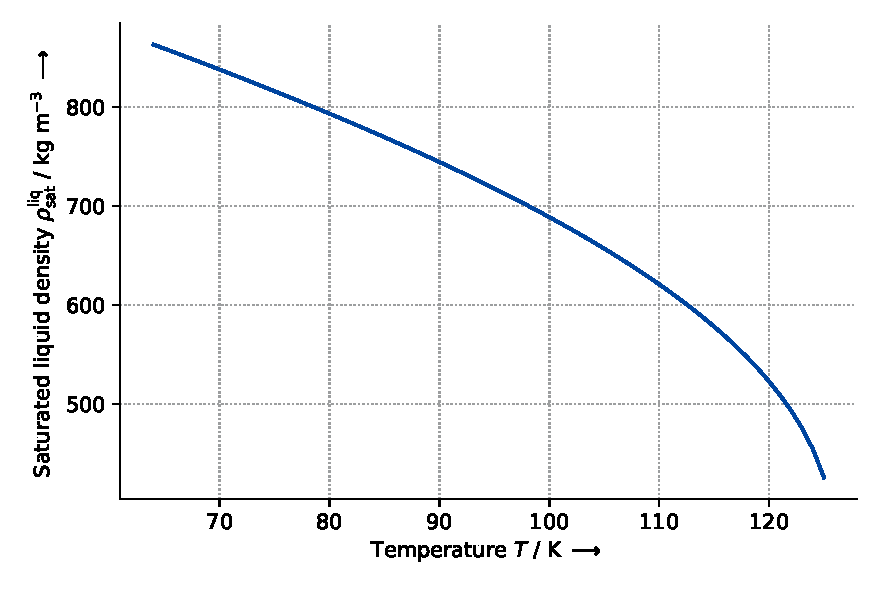
\includegraphics[height=10cm, keepaspectratio]{figs/ref/ref_Nitrogen_SaturatedLiquidDensity_EoS1_1.pdf}}
\end{figure}
%

\FloatBarrier
\newpage
%%%%%%%%%%%%%%%%%%%%%%%%%%%%%%%%%%%%%%%%%%%%%%%%%%%%%%%%%%%%%%%%%%%%%%%%%%%%%%%
%%%%%%%%%%%%%%%%%%%%%%%%%%%%%%%%%%%%%%%%%%%%%%%%%%%%%%%%%%%%%%%%%%%%%%%%%%%%%%%
\subsection{Saturated Liquid Density - EoS1 - ID 2}
%
\begin{tabular}[l]{|lp{11.5cm}|}
\hline
\addlinespace

\textbf{Name:} & Nitrogen \\
\textbf{Equation:} & SaturatedLiquidDensity\_EoS1 \\
\textbf{ID:} & 2 \\
\textbf{Reference:} & Verein Deutscher Ingenieure (2010): VDI Heat Atlas. 2. Ed. Heidelberg: Springer. Online: http://dx.doi.org/10.1007/978-3-540-77877-6. \\
\textbf{Comment:} & None \\

\addlinespace
\hline
\end{tabular}
\newline

\textbf{Equation and parameters:}
\newline
%
Saturated liquid density $\rho_\mathrm{sat}^\mathrm{liq}$ in $\si{\kilogram\per\cubic\meter}$ is calculated depending on temperature $T$ in $\si{\kelvin}$ by:
%
\begin{equation*}
\begin{split}
\rho_\mathrm{sat}^\mathrm{liq} &=& \begin{cases} \rho_\mathrm{ref} \exp(\Omega) & \quad \text{if flag } < 0 \\ \rho_\mathrm{ref} \Omega & \quad \text{else} \end{cases} & \quad\text{, with} \\
\Omega &=& \sum_{i=1}^{8} a_i \xi^{b_i} & \quad\text{, and} \\
\xi &=& 1 - \theta & \quad\text{, and} \\
\theta &=& \nicefrac{T}{T_\mathrm{crit}} & \quad\text{.}
\end{split}
\end{equation*}
%
The parameters of the equation are:
%
\begin{longtable}[l]{lll|lll}
\toprule
\addlinespace
\textbf{Par.} & \textbf{Unit} & \textbf{Value} &	\textbf{Par.} & \textbf{Unit} & \textbf{Value} \\
\addlinespace
\midrule
\endhead

\bottomrule
\endfoot
\bottomrule
\endlastfoot
\addlinespace

flag & - & 1.000000000e+00 & $b_4$ & - & 1.000000000e+00 \\
$T_\mathrm{crit}$ & $\si{\kelvin}$ & 1.261900000e+02 & $a_5$ & - & 1.244762939e+00 \\
$\rho_\mathrm{ref}$ & $\si{\kilogram\per\cubic\meter}$ & 3.130000000e+02 & $b_5$ & - & 1.333333333e+00 \\
$a_1$ & - & 1.000000000e+00 & $a_6$ & - & 0.000000000e+00 \\
$b_1$ & - & 0.000000000e+00 & $b_6$ & - & 0.000000000e+00 \\
$a_2$ & - & 1.504544409e+00 & $a_7$ & - & 0.000000000e+00 \\
$b_2$ & - & 3.500000000e-01 & $b_7$ & - & 0.000000000e+00 \\
$a_3$ & - & 1.575880831e+00 & $a_8$ & - & 0.000000000e+00 \\
$b_3$ & - & 6.666666667e-01 & $b_8$ & - & 0.000000000e+00 \\
$a_4$ & - & -1.790635463e+00 & & & \\

\addlinespace\end{longtable}

\textbf{Validity:}
\newline
Equation is approximately valid for $63.151 \si{\kelvin} \leq T \leq 126.19 \si{\kelvin}$.
\newline

\textbf{Visualization:}
%
\begin{figure}[!htp]
{\noindent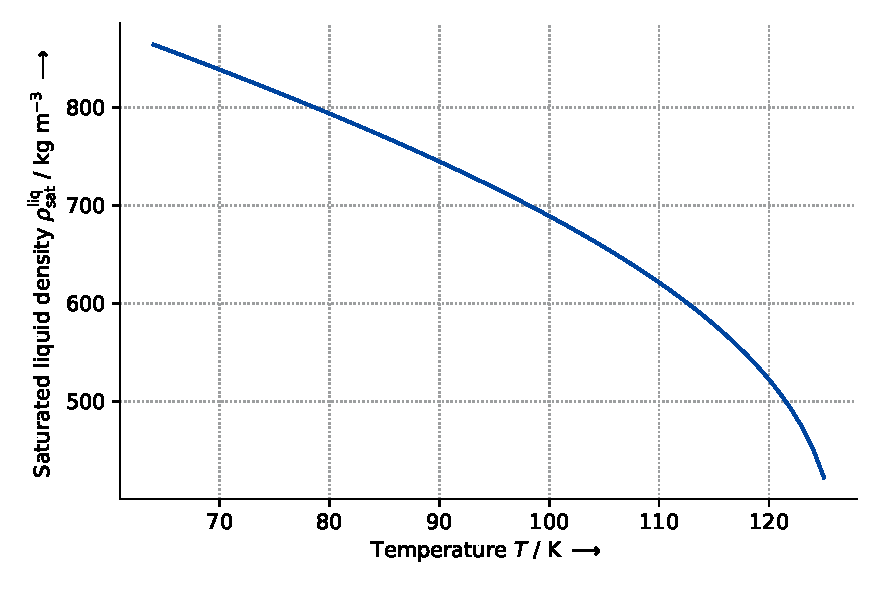
\includegraphics[height=10cm, keepaspectratio]{figs/ref/ref_Nitrogen_SaturatedLiquidDensity_EoS1_2.pdf}}
\end{figure}
%

\FloatBarrier
\newpage
%%%%%%%%%%%%%%%%%%%%%%%%%%%%%%%%%%%%%%%%%%%%%%%%%%%%%%%%%%%%%%%%%%%%%%%%%%%%%%%
%%%%%%%%%%%%%%%%%%%%%%%%%%%%%%%%%%%%%%%%%%%%%%%%%%%%%%%%%%%%%%%%%%%%%%%%%%%%%%%
\subsection{Vapor Pressure - Antoine - ID 1}
%
\begin{tabular}[l]{|lp{11.5cm}|}
\hline
\addlinespace

\textbf{Name:} & Nitrogen \\
\textbf{Equation:} & VaporPressure\_Antoine \\
\textbf{ID:} & 1 \\
\textbf{Reference:} & P.J. Linstrom and W.G. Mallard, Eds., NIST Chemistry WebBook, NIST Standard Reference Database Number 69, National Institute of Standards and Technology, Gaithersburg MD, 20899, https://doi.org/10.18434/T4D303. \\
\textbf{Comment:} & None \\

\addlinespace
\hline
\end{tabular}
\newline

\textbf{Equation and parameters:}
\newline
%
Vapor pressure $p_\mathrm{sat}$ in $\si{\pascal}$ is calculated depending on temperature $T$ in $\si{\kelvin}$ by:
%
\begin{equation*}
\nicefrac{p_\mathrm{sat}}{100000} = 10^{a - \nicefrac{b}{T + c}}
\end{equation*}
%
The parameters of the equation are:
%
\begin{longtable}[l]{lll|lll}
\toprule
\addlinespace
\textbf{Par.} & \textbf{Unit} & \textbf{Value} &	\textbf{Par.} & \textbf{Unit} & \textbf{Value} \\
\addlinespace
\midrule
\endhead

\bottomrule
\endfoot
\bottomrule
\endlastfoot
\addlinespace

$a$ & - & 3.736200000e+00 & $c$ & $\si{\kelvin}$  & -6.788000000e+00 \\
$b$ & $\si{\kelvin}$ & 2.646510000e+02 & & & \\

\addlinespace\end{longtable}

\textbf{Validity:}
\newline
Equation is approximately valid for $63.14 \si{\kelvin} \leq T \leq 126.0 \si{\kelvin}$.
\newline

\textbf{Visualization:}
%
\begin{figure}[!htp]
{\noindent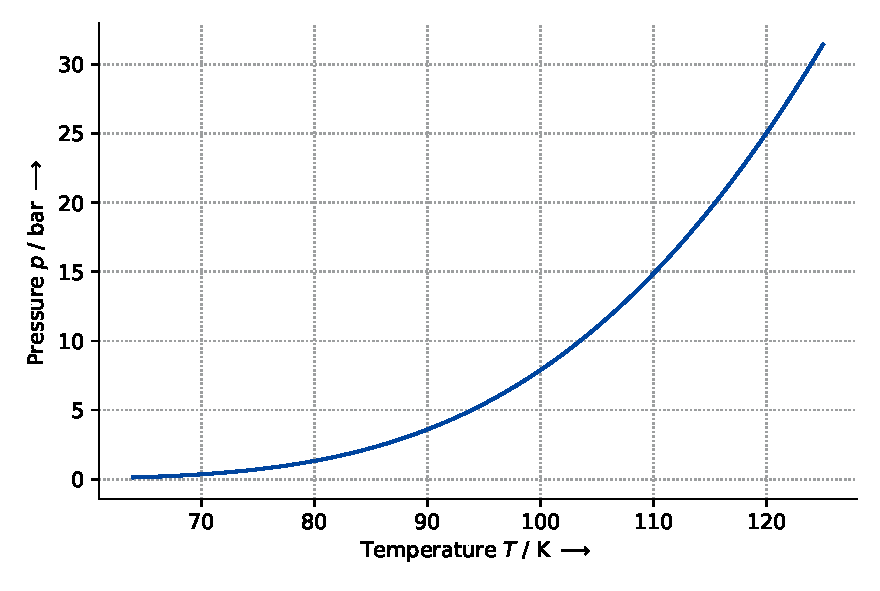
\includegraphics[height=10cm, keepaspectratio]{figs/ref/ref_Nitrogen_VaporPressure_Antoine_1.pdf}}
\end{figure}
%

\FloatBarrier
\newpage
%%%%%%%%%%%%%%%%%%%%%%%%%%%%%%%%%%%%%%%%%%%%%%%%%%%%%%%%%%%%%%%%%%%%%%%%%%%%%%%
%%%%%%%%%%%%%%%%%%%%%%%%%%%%%%%%%%%%%%%%%%%%%%%%%%%%%%%%%%%%%%%%%%%%%%%%%%%%%%%
\subsection{Vapor Pressure - Antoine - ID 2}
%
\begin{tabular}[l]{|lp{11.5cm}|}
\hline
\addlinespace

\textbf{Name:} & Nitrogen \\
\textbf{Equation:} & VaporPressure\_Antoine \\
\textbf{ID:} & 2 \\
\textbf{Reference:} & P.J. Linstrom and W.G. Mallard, Eds., NIST Chemistry WebBook, NIST Standard Reference Database Number 69, National Institute of Standards and Technology, Gaithersburg MD, 20899, https://doi.org/10.18434/T4D303. \\
\textbf{Comment:} & None \\

\addlinespace
\hline
\end{tabular}
\newline

\textbf{Equation and parameters:}
\newline
%
Vapor pressure $p_\mathrm{sat}$ in $\si{\pascal}$ is calculated depending on temperature $T$ in $\si{\kelvin}$ by:
%
\begin{equation*}
\nicefrac{p_\mathrm{sat}}{100000} = 10^{a - \nicefrac{b}{T + c}}
\end{equation*}
%
The parameters of the equation are:
%
\begin{longtable}[l]{lll|lll}
\toprule
\addlinespace
\textbf{Par.} & \textbf{Unit} & \textbf{Value} &	\textbf{Par.} & \textbf{Unit} & \textbf{Value} \\
\addlinespace
\midrule
\endhead

\bottomrule
\endfoot
\bottomrule
\endlastfoot
\addlinespace

$a$ & - & 3.637920000e+00 & $c$ & $\si{\kelvin}$  & -6.344000000e+00 \\
$b$ & $\si{\kelvin}$ & 2.578770000e+02 & & & \\

\addlinespace\end{longtable}

\textbf{Validity:}
\newline
Equation is approximately valid for $63.14 \si{\kelvin} \leq T \leq 78.0 \si{\kelvin}$.
\newline

\textbf{Visualization:}
%
\begin{figure}[!htp]
{\noindent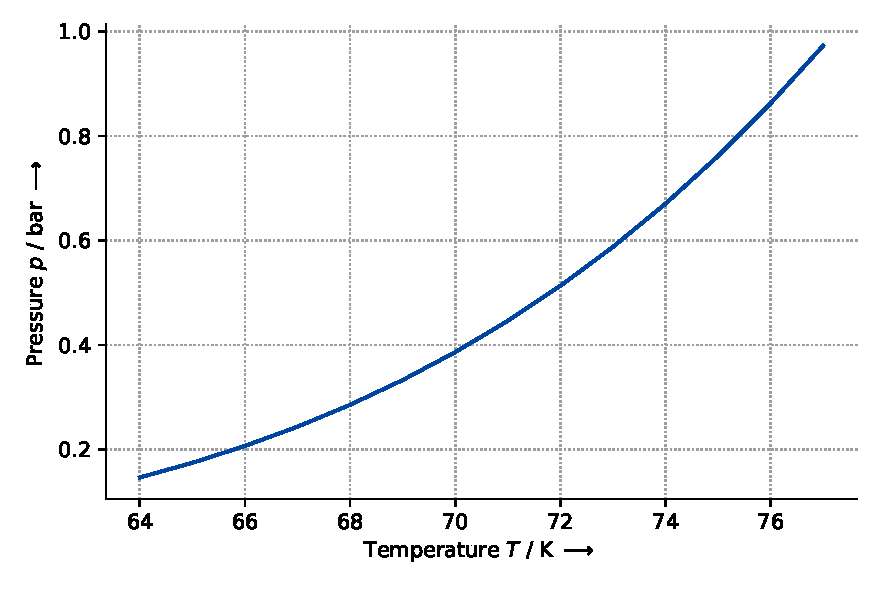
\includegraphics[height=10cm, keepaspectratio]{figs/ref/ref_Nitrogen_VaporPressure_Antoine_2.pdf}}
\end{figure}
%

\FloatBarrier
\newpage
%%%%%%%%%%%%%%%%%%%%%%%%%%%%%%%%%%%%%%%%%%%%%%%%%%%%%%%%%%%%%%%%%%%%%%%%%%%%%%%
%%%%%%%%%%%%%%%%%%%%%%%%%%%%%%%%%%%%%%%%%%%%%%%%%%%%%%%%%%%%%%%%%%%%%%%%%%%%%%%
\subsection{Vapor Pressure - EoS1 - ID 1}
%
\begin{tabular}[l]{|lp{11.5cm}|}
\hline
\addlinespace

\textbf{Name:} & Nitrogen \\
\textbf{Equation:} & VaporPressure\_EoS1 \\
\textbf{ID:} & 1 \\
\textbf{Reference:} & Span, Roland; Lemmon, Eric W.; Jacobsen, Richard T.; Wagner, Wolfgang; Yokozeki, Akimichi (2000): A Reference Equation of State for the Thermodynamic Properties of Nitrogen for Temperatures from 63.151 to 1000 K and Pressures to 2200 MPa. In: Journal of Physical and Chemical Reference Data 29 (6), S. 1361–1433. DOI: 10.1063/1.1349047. \\
\textbf{Comment:} & None \\

\addlinespace
\hline
\end{tabular}
\newline

\textbf{Equation and parameters:}
\newline
%
Vapor pressure $p_\mathrm{sat}$ in $\si{\pascal}$ is calculated depending on temperature $T$ in $\si{\kelvin}$ by:
%
\begin{equation*}
\begin{split}
p_\mathrm{sat} &=& p_\mathrm{crit} \exp \left( \nicefrac{1}{\theta} \sum_{i=1}^{7} a_i \xi^{b_i} \right) & \quad\text{, and} \\
\xi &=& 1 - \theta & \quad\text{, and} \\
\theta &=& \nicefrac{T}{T_\mathrm{crit}} & \quad\text{.}
\end{split}
\end{equation*}
%
The parameters of the equation are:
%
\begin{longtable}[l]{lll|lll}
\toprule
\addlinespace
\textbf{Par.} & \textbf{Unit} & \textbf{Value} &	\textbf{Par.} & \textbf{Unit} & \textbf{Value} \\
\addlinespace
\midrule
\endhead

\bottomrule
\endfoot
\bottomrule
\endlastfoot
\addlinespace

$T_\mathrm{crit}$ & $\si{\kelvin}$ & 1.261920000e+02 & $a_4$ & - & -1.775705640e+00 \\
$p_\mathrm{crit}$ & $\si{\pascal}$ & 3.395800000e+06 & $b_4$ & - & 5.000000000e+00 \\
$a_1$ & - & -6.124452840e+00 & $a_5$ & - & 0.000000000e+00 \\
$b_1$ & - & 1.000000000e+00 & $b_5$ & - & 0.000000000e+00 \\
$a_2$ & - & 1.263272200e+00 & $a_6$ & - & 0.000000000e+00 \\
$b_2$ & - & 1.500000000e+00 & $b_6$ & - & 0.000000000e+00 \\
$a_3$ & - & -7.659100820e-01 & $a_7$ & - & 0.000000000e+00 \\
$b_3$ & - & 2.500000000e+00 & $b_7$ & - & 0.000000000e+00 \\

\addlinespace\end{longtable}

\textbf{Validity:}
\newline
Equation is approximately valid for $63.151 \si{\kelvin} \leq T \leq 126.192 \si{\kelvin}$.
\newline

\textbf{Visualization:}
%
\begin{figure}[!htp]
{\noindent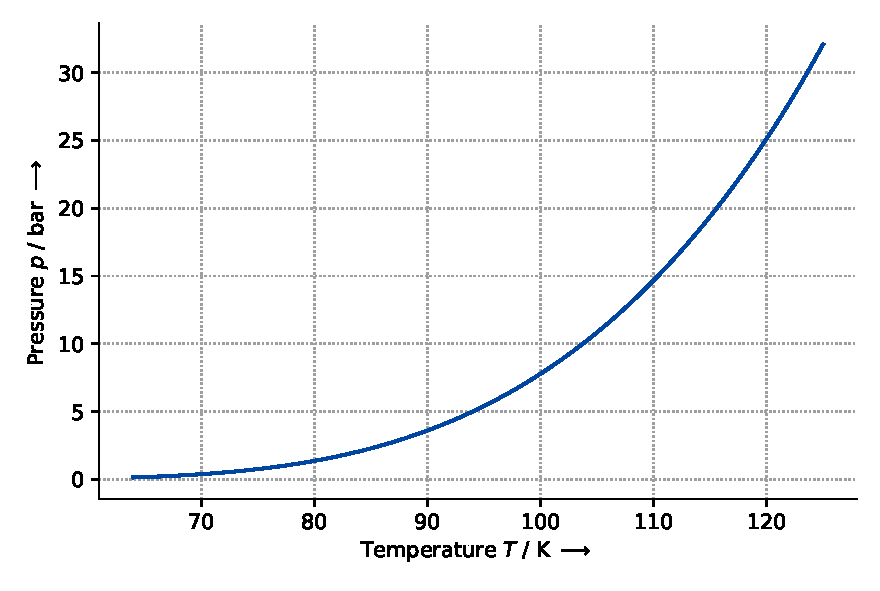
\includegraphics[height=10cm, keepaspectratio]{figs/ref/ref_Nitrogen_VaporPressure_EoS1_1.pdf}}
\end{figure}
%

\FloatBarrier
\newpage
%%%%%%%%%%%%%%%%%%%%%%%%%%%%%%%%%%%%%%%%%%%%%%%%%%%%%%%%%%%%%%%%%%%%%%%%%%%%%%%
%%%%%%%%%%%%%%%%%%%%%%%%%%%%%%%%%%%%%%%%%%%%%%%%%%%%%%%%%%%%%%%%%%%%%%%%%%%%%%%
\subsection{Vapor Pressure - EoS1 - ID 2}
%
\begin{tabular}[l]{|lp{11.5cm}|}
\hline
\addlinespace

\textbf{Name:} & Nitrogen \\
\textbf{Equation:} & VaporPressure\_EoS1 \\
\textbf{ID:} & 2 \\
\textbf{Reference:} & Verein Deutscher Ingenieure (2010): VDI Heat Atlas. 2. Ed. Heidelberg: Springer. Online: http://dx.doi.org/10.1007/978-3-540-77877-6. \\
\textbf{Comment:} & None \\

\addlinespace
\hline
\end{tabular}
\newline

\textbf{Equation and parameters:}
\newline
%
Vapor pressure $p_\mathrm{sat}$ in $\si{\pascal}$ is calculated depending on temperature $T$ in $\si{\kelvin}$ by:
%
\begin{equation*}
\begin{split}
p_\mathrm{sat} &=& p_\mathrm{crit} \exp \left( \nicefrac{1}{\theta} \sum_{i=1}^{7} a_i \xi^{b_i} \right) & \quad\text{, and} \\
\xi &=& 1 - \theta & \quad\text{, and} \\
\theta &=& \nicefrac{T}{T_\mathrm{crit}} & \quad\text{.}
\end{split}
\end{equation*}
%
The parameters of the equation are:
%
\begin{longtable}[l]{lll|lll}
\toprule
\addlinespace
\textbf{Par.} & \textbf{Unit} & \textbf{Value} &	\textbf{Par.} & \textbf{Unit} & \textbf{Value} \\
\addlinespace
\midrule
\endhead

\bottomrule
\endfoot
\bottomrule
\endlastfoot
\addlinespace

$T_\mathrm{crit}$ & $\si{\kelvin}$ & 1.261900000e+02 & $a_4$ & - & -1.781730000e+00 \\
$p_\mathrm{crit}$ & $\si{\pascal}$ & 3.396000000e+06 & $b_4$ & - & 5.000000000e+00 \\
$a_1$ & - & -6.124980000e+00 & $a_5$ & - & 0.000000000e+00 \\
$b_1$ & - & 1.000000000e+00 & $b_5$ & - & 0.000000000e+00 \\
$a_2$ & - & 1.264990000e+00 & $a_6$ & - & 0.000000000e+00 \\
$b_2$ & - & 1.500000000e+00 & $b_6$ & - & 0.000000000e+00 \\
$a_3$ & - & -7.676500000e-01 & $a_7$ & - & 0.000000000e+00 \\
$b_3$ & - & 2.500000000e+00 & $b_7$ & - & 0.000000000e+00 \\

\addlinespace\end{longtable}

\textbf{Validity:}
\newline
Equation is approximately valid for $63.151 \si{\kelvin} \leq T \leq 126.19 \si{\kelvin}$.
\newline

\textbf{Visualization:}
%
\begin{figure}[!htp]
{\noindent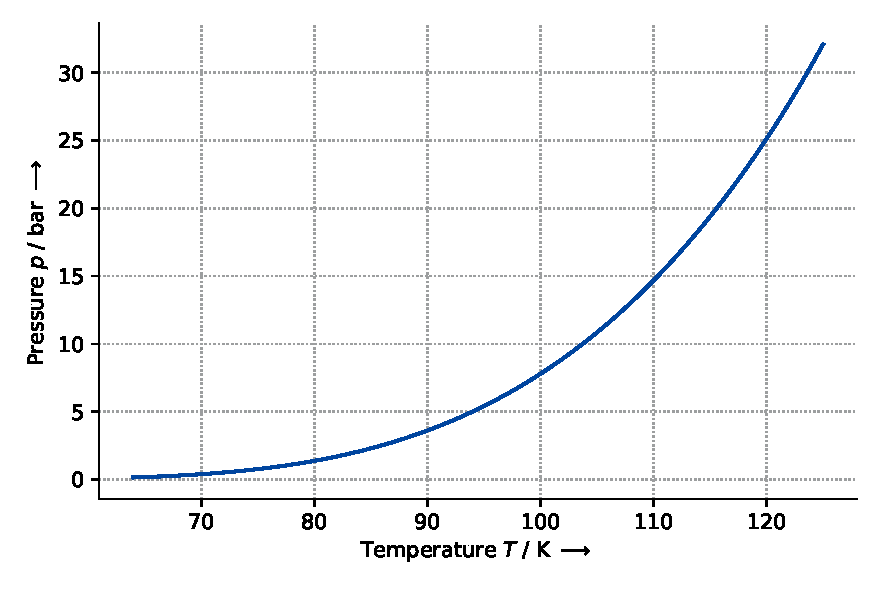
\includegraphics[height=10cm, keepaspectratio]{figs/ref/ref_Nitrogen_VaporPressure_EoS1_2.pdf}}
\end{figure}
%

\FloatBarrier
\newpage
%%%%%%%%%%%%%%%%%%%%%%%%%%%%%%%%%%%%%%%%%%%%%%%%%%%%%%%%%%%%%%%%%%%%%%%%%%%%%%%
%%%%%%%%%%%%%%%%%%%%%%%%%%%%%%%%%%%%%%%%%%%%%%%%%%%%%%%%%%%%%%%%%%%%%%%%%%%%%%%
\subsection{Vapor Pressure - EoSCubic - ID 1}
%
\begin{tabular}[l]{|lp{11.5cm}|}
\hline
\addlinespace

\textbf{Name:} & Nitrogen \\
\textbf{Equation:} & VaporPressure\_EoSCubic \\
\textbf{ID:} & 1 \\
\textbf{Reference:} & Lemmon, E. W.; Bell, I. H.; Huber, M. L.; McLinden, M. O. (2018): NIST Standard Reference Database 23. Reference Fluid Thermodynamic and Transport Properties-REFPROP, Version 10.0, National Institute of Standards and Technology. Online: https://www.nist.gov/srd/refprop. \\
\textbf{Comment:} & None \\

\addlinespace
\hline
\end{tabular}
\newline

\textbf{Equation and parameters:}
\newline
%
Vapor pressure $p_\mathrm{sat}$ in $\si{\pascal}$ is calculated depending on temperature $T$ in $\si{\kelvin}$ and molar volume v in $\si{\mole\per\cubic\meter}$ by using cubic equation of state. For this purpose, molar volumes of liquid and vapor phase are changed iteratively until fugacity coefficients of vapor and liquid phase are equal. Cubic equation of state is given by:
\begin{equation*}
\begin{split}
p &=& R \frac{T}{v - b} - \frac{a}{v \left(v + b\right)} & \quad\text{, and} \\
a &=& \frac{1}{9 \left(2^{\nicefrac{1}{3}} - 1\right)} \frac{\left(R T_\mathrm{crit} \right)^2}{p_\mathrm{crit}} \alpha & \quad\text{, and} \\
b &=& 0.08664 R \frac{T_\mathrm{crit}}{p_\mathrm{crit}} & \quad\text{, and} \\
\alpha &=& \left(1 + \kappa \left(1 - \sqrt(\nicefrac{T}{T_\mathrm{crit}}) \right) \right)^2 & \quad\text{, and} \\
\kappa &=& 0.48508 + 1.55171 \omega - 0.15613 \omega^2 & \quad\text{.}
\end{split}
\end{equation*}
%
The parameters of the equation are:
%
\begin{longtable}[l]{lll|lll}
\toprule
\addlinespace
\textbf{Par.} & \textbf{Unit} & \textbf{Value} &	\textbf{Par.} & \textbf{Unit} & \textbf{Value} \\
\addlinespace
\midrule
\endhead

\bottomrule
\endfoot
\bottomrule
\endlastfoot
\addlinespace

EoS & - & -5.000000000e+00 & $\beta_0$ & - & 0.000000000e+00 \\
$T_\mathrm{crit}$ & $\si{\kelvin}$ & 1.261900000e+02 & $\beta_1$ & - & 0.000000000e+00 \\
$p_\mathrm{crit}$ & $\si{\pascal}$ & 3.395800000e+06 & $\beta_2$ & - & 0.000000000e+00 \\
$\omega$ & - & 3.720000000e-02 & $\beta_3$ & - & 0.000000000e+00 \\
$\kappa_1$ & - & 0.000000000e+00 & & & \\

\addlinespace\end{longtable}

\textbf{Validity:}
\newline
Equation is approximately valid for $72.62365 \si{\kelvin} \leq T \leq 107.2615 \si{\kelvin}$.
\newline

\textbf{Visualization:}
%
\begin{figure}[!htp]
{\noindent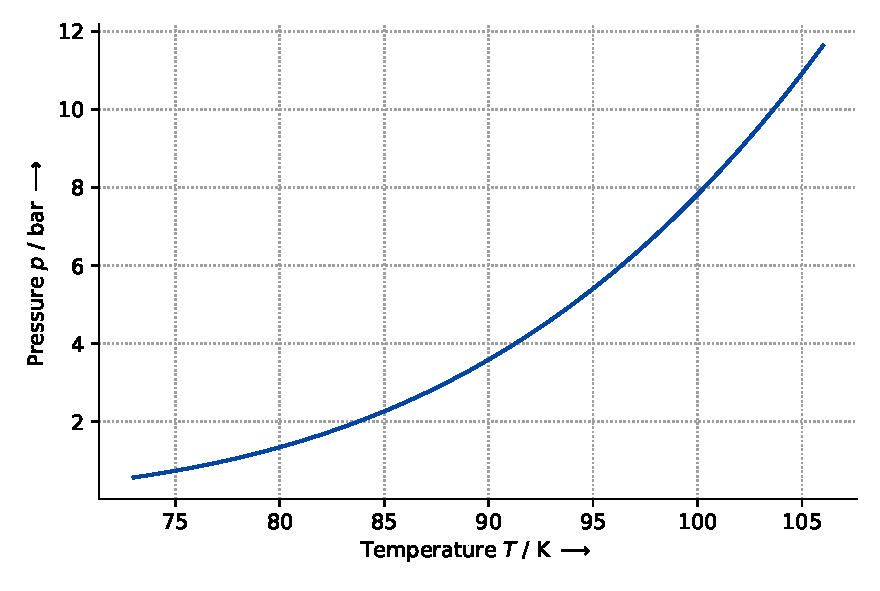
\includegraphics[height=10cm, keepaspectratio]{figs/ref/ref_Nitrogen_VaporPressure_EoSCubic_1.pdf}}
\end{figure}
%

\FloatBarrier
\newpage
%%%%%%%%%%%%%%%%%%%%%%%%%%%%%%%%%%%%%%%%%%%%%%%%%%%%%%%%%%%%%%%%%%%%%%%%%%%%%%%
%%%%%%%%%%%%%%%%%%%%%%%%%%%%%%%%%%%%%%%%%%%%%%%%%%%%%%%%%%%%%%%%%%%%%%%%%%%%%%%
\subsection{Vapor Pressure - EoSCubic - ID 2}
%
\begin{tabular}[l]{|lp{11.5cm}|}
\hline
\addlinespace

\textbf{Name:} & Nitrogen \\
\textbf{Equation:} & VaporPressure\_EoSCubic \\
\textbf{ID:} & 2 \\
\textbf{Reference:} & Lemmon, E. W.; Bell, I. H.; Huber, M. L.; McLinden, M. O. (2018): NIST Standard Reference Database 23. Reference Fluid Thermodynamic and Transport Properties-REFPROP, Version 10.0, National Institute of Standards and Technology. Online: https://www.nist.gov/srd/refprop. \\
\textbf{Comment:} & None \\

\addlinespace
\hline
\end{tabular}
\newline

\textbf{Equation and parameters:}
\newline
%
Vapor pressure $p_\mathrm{sat}$ in $\si{\pascal}$ is calculated depending on temperature $T$ in $\si{\kelvin}$ and molar volume v in $\si{\mole\per\cubic\meter}$ by using cubic equation of state. For this purpose, molar volumes of liquid and vapor phase are changed iteratively until fugacity coefficients of vapor and liquid phase are equal. Cubic equation of state is given by:
\begin{equation*}
\begin{split}
p &=& R \frac{T}{v - b} - \frac{a}{v \left(v + b\right) + b \left(v - b\right)} & \quad\text{, and} \\
a &=& 0.45724 \frac{\left(R T_\mathrm{crit} \right)^2}{p_\mathrm{crit}} \alpha & \quad\text{, and} \\
b &=& 0.07780 R \frac{T_\mathrm{crit}}{p_\mathrm{crit}} & \quad\text{, and} \\
\alpha &=& \left(1 + \kappa \left(1 - \sqrt(\nicefrac{T}{T_\mathrm{crit}}) \right) \right)^2 & \quad\text{, and} \\
\kappa &=& 0.37464 + 1.54226 \omega - 0.26992 \omega^2 & \quad\text{.}
\end{split}
\end{equation*}
%
The parameters of the equation are:
%
\begin{longtable}[l]{lll|lll}
\toprule
\addlinespace
\textbf{Par.} & \textbf{Unit} & \textbf{Value} &	\textbf{Par.} & \textbf{Unit} & \textbf{Value} \\
\addlinespace
\midrule
\endhead

\bottomrule
\endfoot
\bottomrule
\endlastfoot
\addlinespace

EoS & - & 1.000000000e+01 & $\beta_0$ & - & 0.000000000e+00 \\
$T_\mathrm{crit}$ & $\si{\kelvin}$ & 1.261900000e+02 & $\beta_1$ & - & 0.000000000e+00 \\
$p_\mathrm{crit}$ & $\si{\pascal}$ & 3.395800000e+06 & $\beta_2$ & - & 0.000000000e+00 \\
$\omega$ & - & 3.720000000e-02 & $\beta_3$ & - & 0.000000000e+00 \\
$\kappa_1$ & - & 0.000000000e+00 & & & \\

\addlinespace\end{longtable}

\textbf{Validity:}
\newline
Equation is approximately valid for $72.62365 \si{\kelvin} \leq T \leq 107.2615 \si{\kelvin}$.
\newline

\textbf{Visualization:}
%
\begin{figure}[!htp]
{\noindent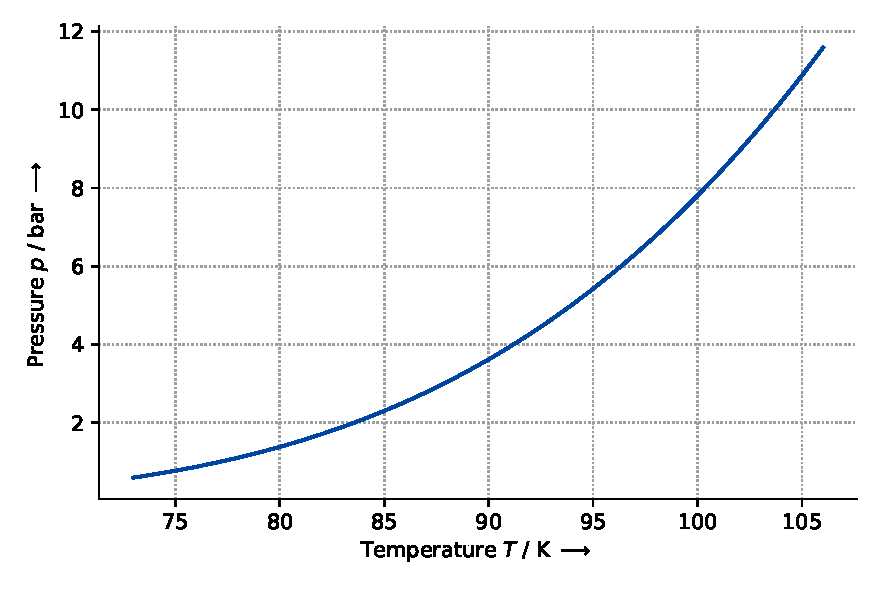
\includegraphics[height=10cm, keepaspectratio]{figs/ref/ref_Nitrogen_VaporPressure_EoSCubic_2.pdf}}
\end{figure}
%

\FloatBarrier
\newpage
%%%%%%%%%%%%%%%%%%%%%%%%%%%%%%%%%%%%%%%%%%%%%%%%%%%%%%%%%%%%%%%%%%%%%%%%%%%%%%%
